\documentclass[conference]{IEEEtran}

\usepackage{graphicx}
\usepackage{subfigure}


\hyphenation{op-tical net-works semi-conduc-tor}


\begin{document}
%
% paper title
% can use linebreaks \\ within to get better formatting as desired
\title{Better JavaScript Runtime Understanding by Automatic Function Naming}


% author names and affiliations
% use a multiple column layout for up to three different
% affiliations
\author{\IEEEauthorblockN{Salman Mirghasemi}
\IEEEauthorblockA{\'Ecole Polytechnique F\'ed\'erale de Lausanne\\
Lausanne, Switzerland\\
salman.mirghasemi@epfl.ch}
\and
\IEEEauthorblockN{John J. Barton}
\IEEEauthorblockA{IBM Research - Almaden\\
San Jose, USA\\
johnjbarton@johnjbarton.com}
\and
\IEEEauthorblockN{Claude Petitpierre}
\IEEEauthorblockA{\'Ecole Polytechnique F\'ed\'erale de Lausanne\\
Lausanne, Switzerland\\
claude.petitpierre@epfl.ch}}
\maketitle


\begin{abstract}
%\boldmath
%Understanding runtime elments play a key role in program comprehension. In dynamic weak-typed languages like JavaScript, runtime elements are mainly concrete values that tell a little about their meta data and structure. This dynamic languages feature makes their understanding hard.
\end{abstract}



\section{Introduction}
Today JavaScript has a unique role in web programming, considered as the web assembly language. This language is used by 97 out of the web's 100 most popular sites\footnote[1]{http://www.alexa.com}.It is very likely that JavaScript keeps this critical role at least for the next few years. Along with the growth of demands for more comprehensive user interfaces, the size and the complexity of web applications is increasing. Morover, JavaScript is also becoming a general purpose computing platform with office applications[], browsers[], server-side applications[] and development environments \cite{Ingalls} being developed in JavaScript.

JavaScript developers have to improve their develoment processes and practices to cope with these fast changes. They need modern editors for writing and editing larger programs and effective tools for understanding complicated JavaScript runtime. However, there has been severe inherent barriers for improving JavaScript tool support. 
Unlike many traditional object oriented languages such as Java and C\#, it does not have classes, and does not encourage encapsulation or even structured programming JavaScript is a weakly typed language with no type declarations and only run-time checking of calls and field accesses \cite{Richards}. It means that the code contains less data about JavaScript elements and how they are related. For example, a variable value can be primitive values, objects with any structure or even a function. Therefore, lack of describing data in JavaScript code is a fundamental issue in enhancing tools.

Catching errors early (i.e., before or at the time of compilation) is an important feature for editors. It can saves developers' time, prevents bugs and improves the program reliability. However, many errors can not be recognized without a strong typing stystem. To attack this issue a few static typing systems have been proposed for JavaScript \cite{Anderson, Anderson2, Heidegger, Thiemann}. These approaches analyze source codes and deduce possible values and object structures based on possible program control flows lead to assignment to a variable. The discovered facts about variables are not only useful for catching errors but to provide modern editors' features such as auto-complete and refactoring. 

Although the mentioned approaches are able to recognize errors or provide modern editing features by the the discovered facts about JavaScript elements, they do not have means to transform this information to the developer. For example, objects are not associated to classes in JavaScript, and no structure can be assumed by the developer.
If it is discovered that a variable value is only constructed by a specific function, this information can also be shared with the developer. The function can work like a class and gives some cue to the developer about the object structure. However, due to dynamic nature of JavaScript many elements have no identifier. Therefore, even in the cases that the constructor of an object is known, it can not be presented because the constructor has no identifier or the identifier is not recognizable for the developer.

% about JavaScript elements less explicit meta data for the code exist is available to editors and tools for program verifiction, 

As a consequence, the information provided in editors and tools for JavaScript elements is usually limited and doesn't give enough hint for rapid recall to developers. 
Understanding runtime elments play a key role in program comprehension.
In dynamic weak-typed languages like JavaScript, runtime elements are
only concrete values that tell a little about their meta data and structure.
This dynamic languages feature makes their understanding hard.

%For example to know an object, developer has to examine the object properties and from the property names and values, some connections
%understanding JavaScript code and its runtime is much harder for developers.


\section{The Function Naming Problem}
Figure~\ref{debuggers} shows the call stack view of two famous JavaScript debuggers, Firebug and Google Chrome , paused at the same breakpoint. The differences between two call stack, particularly in the first two frames, are due to different implementations of event handling in the underlying platforms. Google chrome shows \texttt{anonymouse} for three functions which doesn't give any useful information to the developer. The developer has to look at the specified source file and line number to recall the function. Although Firebug shows more function names, it is also unsuccessful about one function. 
 

%___ why it is hard
%-- Check here: http://kangax.github.com/nfe/
%___ The importance of having function names
%___ related work for type system

\begin{figure*}[htp]
\centerline{
\subfigure[Firefox Firebug Debugger]{\label{fig_first_case}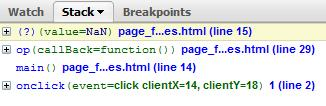
\includegraphics[width=.47\textwidth]{fbug-callstack.jpg}}
\hfil
\subfigure[Google Chrome Debugger]{\label{fig_second_case}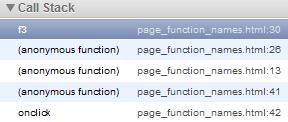
\includegraphics[width=0.47\textwidth]{chrome-callstack.jpg}}}
\caption{These two figures show the call stack view of Firebug and Google Chrome JavaScript debuggers paused at the same point. 
The Google Chrome debugger is unable to find three function names and The Firebug debugger fails at one case.}
\label{debuggers}
\end{figure*}

The importance of function names is not limited only to call stack view. A function can be used as a constructor for creating new objects. The constructor name like class name in traditional languages such as Java, can be used in object representation. It can help developer in understanding the structure and role of object without looking into its properties.



\section{Automatic Funcation Naming}

%explain function expression and function declerations
%moreover explain creation of the list of outer scopes.

\subsection{A Global Name for a Function Object}

\begin{figure}[htp]
\begin{verbatim}
(a) Case 1:
 function foo(){ ... }

(b) Case 2:
 var foo = function { ... } 
 
(c) Case 3:
 var foo = {
     bar : function { ...}
 }

(d) Case 4:

 var foo = function(){
           ....
           return function(){ ... }
 }()
 
(e) Case 5:
 var foo = function(){ 
 					 return ...;
 }()					
 
(f) Case 6:
 var foo = function(){
 
 }()();
 
(g)
 foo(function(){ ... });
 
(h)
 array = [...., function(){},...]
 
(i)
 array[i] = function(){};   

\end{verbatim}
\caption{Different cases of function object creation.}
\label{fig:functionCreation}
\end{figure}

\subsection{Naming Functions in Call Stack}


\section{Related Work}
%Another strand of research has tried to investigate how to provide better tools for developers for catching errors early. Being a weakly typed language with no type declarations and only run-time checking of calls and field accesses, it is natural to try to provide a static type system for JavaScript [2, 1, 3, 24, 13]. Finally, after many years of neglect, modern implementations of JavaScript have started to appear which use state of the art just-in-time compilation techniques [10].

%For JavaScript, Anderson et al. proposed a type system with definite and potential types [2, 1, 3], while Heidegger and Thiemann following up on some of their earlier work [24, 18] propose recency types in [13], and Furr et al. proposed a related system for DRuby [9]. While all of these type systems acknowledge some minor simplifications to the target language, they rely on fairly similar assumptions. For instance, Thiemann writes: �Usually, no further properties are defined after the initialization and the type of the properties rarely changes.� This suggests that object types are stable at run-time and can be described using, e.g., traditional rowtypes. In fact all the proposals take the view that an object�s type should be the sum of all possible fields and methods that it could contain, with some of them being undefined; they differ mostly on how to perform strong updates to avoid polluting all properties with undefined values. Interestingly, language implementors make similar assumptions. For instance, Google�s V8 JavaScript engine is reported to optimistically associate �classes� to objects on the assumption that their shape will not change too much, though with a fallback case for highly dynamic objects 3. This design is similar to implementations of one of JavaScript�s influences, Self [5], and is expected to work for the same reasons. As the above mentioned hypothesis is crucial for the applicability and usefulness of the results, it deserves careful study. In fact, we have found a number of similar assumptions in the literature which we list below.We first review the salient features of the language to provide sufficient background for readers unfamiliar with JavaScript.

\section{Conclusion}
In this paper we presented an approach for naming JavaScript functions both
as individual objects and in call stack. 


\begin{thebibliography}{10}

\bibitem{IEEEhowto:kopka}
H.~Kopka and P.~W. Daly, \emph{A Guide to \LaTeX}, 3rd~ed.\hskip 1em plus
  0.5em minus 0.4em\relax Harlow, England: Addison-Wesley, 1999.

\bibitem{Anderson}
C. Anderson, P. Giannini, and S. Drossopoulou. \newblock Towards Type Inference for JavaScript.
\newblock In \emph{Proceedings of the 19th European conference on Object-Oriented Programming(ECOOP)},
July, 2005.

\bibitem{Anderson2}
C. Anderson and P. Giannini. \newblock Type checking for javascript.
\newblock \emph{Electr. Notes Theor. Comput. Sci.}, 138(2), 2005. 

\bibitem{ECMA}
ECMA International.
\newblock \emph{ECMA-262: ECMAScript Language Specification},
ECMA (European Association for Standardizing Information
and Communication Systems), Geneva, Switzerland, third edition,
December 1999. 

\bibitem{Heidegger}
P. Heidegger and P. Thiemann.\newblock Recency types for dynamically-typed, object-based languages.
\newblock In \emph{Proceedings of Foundations of Object Oriented Languages (FOOL)},
2009.

\bibitem{Ingalls}
D. Ingalls, K. Palacz, S. Uhler and A. Taivalsaari.\newblock The lively kernel a self-supporting system on
a web page.
\newblock In \emph{Self-Sustaining Systems},
2008.

\bibitem{Richards}
G. Richards, S. Lebresne, B. Burg and J. Vitek.\newblock An analysis of the dynamic behavior of JavaScript programs.
\newblock In \emph{Proceedings of the 2010 ACM SIGPLAN conference on Programming language design and implementation(PLDI)},
June, 2010.

\bibitem{Thiemann}
P. Thiemann.\newblock Towards a type system for analyzing JavaScript programs.
\newblock In \emph{Proceedings of European Symposium on Programming (ESOP)},
2005.


\end{thebibliography}



% that's all folks
\end{document}


